We were offered to use the Crowdboard to help with  need-finding and ideation. The Crowdboard is an augmented white-board, designed and developed at the Helsinki University. The Crowdboard consists of multiple screens whose content is shared online with workers from Amazon Mechanical Turk \footnote{\url{https://www.mturk.com/}}. This enables the Amazon Turk workers to see the notes on the white-board and to post comments on these notes. Figure \ref{fig:crowdboard-diagram} shows a diagram of how the Crowdboard works \cite{crowdboard}. 

\begin{figure}[h]
 \centering
 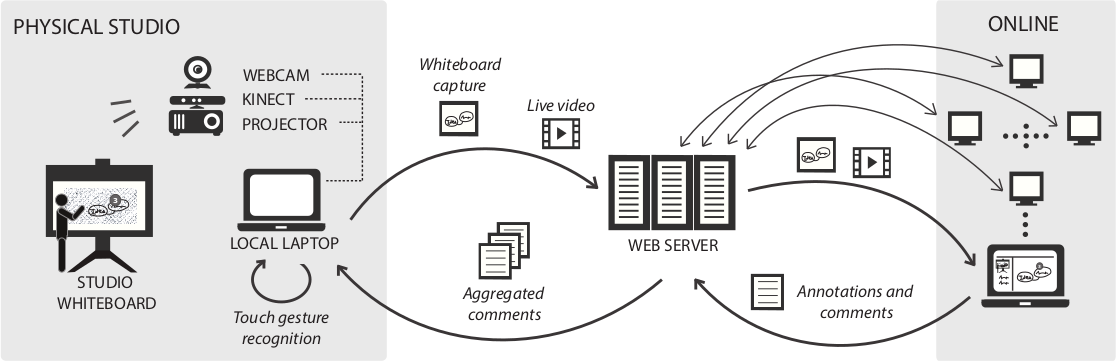
\includegraphics[width=\textwidth]{images/crowdboard-diagram.png}
 \caption{Overview over the Crowdboard's architecture \& information flow \cite{crowdboard}}
 \label{fig:crowdboard-diagram}
\end{figure}

In the Crowdboard session our team had three loosely related goals: we wanted to find out what people are doing in their break-time and what motivates them to take a break. We also wanted to validate our ideas and see if people would be willing to use our system. The final goal was to find out new ideas by pitching rough drafts and gathering ideas. Before doing so, the Amazon Turk workers had to be invited (Appendix 3).

Furthermore, we had to prepare an initial task to Turkers joining the Crowdboard session (Appendix 4).

The experiment took place on the afternoon of March 23, 2017. There were ca. 20 Amazon Turk workers participating in the session. We got around 40 useful comments on the ideas that were discussed. As mentioned before, we had three goals in this session.

The first goal was to find out what people do in their breaks. As we suspected, many people eat something in their break. There were some suggestions on how to make the lunch break more interesting: 3 people suggested having lunch or ordering food together with everyone in the department or, if a kitchen is available, to cook together. Other results of the Crowdboard session include: 
\begin{description}
  \item[Coffee Break] We suspected that coffee breaks are a common break activity. This was verified in multiple interviews and also in this Crowdboard session.
  \item[Board Games] We had the idea for our application to suggest board games as one acitivity to bring colleagues together This suggestion was repeated in the Crowdboard session while another comment suggested to do puzzles or crosswords.
  \item[Waling/Outside breaks] Another suggestion from the session that could be added as an activity in our application.
\end{description}

\begin{comment}
Break Habits
\begin{itemize}
  \item \textsl{Snacking, Lunch, Overeating, Conferences with food}
  \item \textsl{Smoking}
  \item Procrastinating
  \item Reading
  \item Texting
  \item \textsl{Puzzles, Crosswords}
  \item \textsl{Board games, chess or checkers}
  \item \textsl{Go outside, walking break}
  \item Personal or resting break
\end{itemize}
\end{comment}

Since our team consists solely of non-smokers, we did not think of smoking breaks. This was an activity discovered by the Crowdboard session. However, the discussion was primarily focused on the potential health damages. So while smoking is a valid break activity, we will not encourage smoking with our application and suggest other activities instead.
t
Some time into the session, we introduced the idea of suggesting more active breaks, e.g. sports. This idea also attracted some comments including ``people who share a common activity probably develop
connections faster''.

\begin{comment}
would you like to do "active" breaks? sports etc
\begin{itemize}
  \item Setting up a small game table such as table tennis and
holding tournaments
  \item Take walks around the building
  \item stretching
  \item people who share a common activity probably develop
connections faster
\end{itemize}

suggestion of colleagues to take breaks with?
\begin{itemize}
  \item use time to connect with someone new
\end{itemize}
\end{comment}

\begin{comment}
tournaments \& leaderboards
\begin{itemize}
  \item A break room
with games, vending machines, tournament equipment etc
  \item Having on going health bets or competitions
a raffle with reward incentives
  \item free coffee, barnes and nobles gift certificate
  \item You could have people who are partnered up with the
desktop app work together to solve a puzzle for
competition or leaderboards
  \item Jeopardy game using work information
exercise room with interactive gaming like example Wii
  \item Healthy competition will increase happiness too and coherence
\end{itemize}
\end{comment}

The second goal of the Crowdboard session was to find out when or why people take breaks. We were looking for triggers that do not necessarily relate to lunch breaks. The comments on this topic were mostly related to stress, fatigue, or ``getting stuck''. There were only a few comments on this topic.

\begin{comment}
triggers break
\begin{itemize}
  \item When I hit a wall on a project
  \item stress, fatigue, work pressure
  \item not delegating tasks well
  \item no work available
\end{itemize}
\end{comment}

The final goal was to find out if people would use a system that suggests them to take a break with another person and also suggests some activities. The idea to match up different people received positive or neutral comments; one could use the break to ``connect with someone new''. It was also mentioned that ``set breaks would help people take the breaks together''.

We also mentioned the idea of using a ``pressure chair'' to determine how long a user has been working. There was only one useful comment on this idea which suggested to use pressure sensors on the keyboard instead.

All in all, many of our ideas and assumptions were verified in the Crowdboard session. We also got many new insights and were also notified of some things we missed.

\begin{comment}
technology
\begin{itemize}
  \item using an app to coordinate with workers through phones
or computers to alert unannounced breaks
  \item Video games
  \item There could be a desktop app that lets them know they
need to take a break soon based on when they clocked in
for work.
\end{itemize}

set breaks after specific time - 
\begin{itemize}
  \item Set breaks would help people take the breaks together.
\end{itemize}

pressure sensor chair
\begin{itemize}
  \item There should be pressure sensors on the keyboard. It can
identify issues with carpal tunnel
  \item Go green and healthy, it will promote a positive
environment
  \item Yoga room or a work gym where associates can socialize	
  \item An employee lounge will be nice, with a tv, healthy snacks,
using green materials
\end{itemize}
\end{comment}